\section{Quenched arm bounds and compactness of the explorations}
\label{sec:tightness}

The polygon comparison concerns deterministic domains.  To use it after
an exploration, we first need geometric control of the random prefixes.
We obtain that control from the local annulus barriers of~\cite{Q}.
All radii in this section are physical radii, fixed before the mesh
tends to zero.  In particular, the argument does not require an annulus
estimate uniform down to the lattice spacing.

\subsection{Fixing the environment}

Write $\P_{\rm env}$ for probability over the bonds.  Use the
countable stock $\mathscr T$ of collared polygon tests from
Section~\ref{sec:pure}, with its fixed rounding prescriptions,
dual-grid versions, and finite sheet-incidence data.  Its strict-margin
approximation property will allow tests selected from a limiting
geometry to be chosen from this one countable stock.

The second countable collection consists of square annuli of the fixed
ratio in Lemma~\ref{lem:barrier-input}.  Their centers
and inner radii range over dense countable sets; the collection again
includes both colors and the required incident-layer conventions.
Call an annulus good when its quenched probability of an actual radial
crossing is at most $1-c_0$ under the law wiring both rims together.
Here $c_0>0$ is the constant from that lemma.  An actual crossing uses
ordinary open edges; identification of the rims does not itself count
as a crossing.

\begin{lemma}[A deterministic subsequence of environments]
\label{lem:quenched-diagonal}
From every subsequence of the prescribed meshes one can extract a
further deterministic subsequence such that, for
$\P_{\rm env}$-almost every environment, the following hold:
\begin{enumerate}
\item every test in $\mathscr T$ has the pure limiting crossing
probability of Proposition~\ref{prop:pure-four-mark};
\item every fixed annulus in the second collection is eventually good.
\end{enumerate}
\end{lemma}

\begin{proof}
For each fixed polygon, Corollary~\ref{cor:fixed-tests} gives
convergence in environmental probability.  For each fixed physical
annulus, its inner radius in lattice units tends to infinity, so
Lemma~\ref{lem:barrier-input} gives
goodness with probability tending to one.  Enumerate the tests and
annuli.  Choose the $j$th mesh of the further subsequence so that the
probability of an error larger than $1/j$ in any of the first $j$
polygon tests, or failure of goodness for any of the first $j$ annuli,
is at most $2^{-j}$.  The Borel--Cantelli lemma proves the simultaneous
assertions.  Independence between different meshes is not used.
The dual assertions follow in the same way, since the critical odds
duality preserves the law of the environment.
\end{proof}

Until the last paragraph of Section~\ref{sec:identification}, fix an
environment in the full-probability event of this lemma and use $n$
for its further subsequence.  All probabilities henceforth concern FK
configurations in this fixed environment.  Their bounds may depend on
that environment through how small the mesh must be.

For $z\in\C$ and $0<r<R$, let $A(z;r,R)$ denote a Euclidean annulus.
Its lattice version includes an incident layer at each rim.  Write
$\phi^{\rm w}_{n,z;r,R}$ for the full-grid FK law in this annulus,
with both rims wired together, and $\mathcal R_n(z;r,R)$ for its
ordinary radial crossing event.  Either the primal grid with its
odds, or the dual grid with the dual odds, may be used in this notation.

\begin{lemma}[Full-grid arm bound]
\label{lem:full-grid-arm}
For every fixed $R>0$ and bounded set $K\subset\C$,
\begin{equation}\label{eq:full-grid-arm}
 \lim_{r\downarrow0}\limsup_{n\to\infty}
 \sup_{z\in K}
 \phi^{\rm w}_{n,z;r,R}\bigl(\mathcal R_n(z;r,R)\bigr)=0.
\end{equation}
The same conclusion holds for actual arms in subgraphs of the annulus
whose induced boundary partition has no wire attachments away from
the rims, apart from ordinary identifications at the same physical
vertex.  It also bounds the event that an arm occurs in any of a
collection of such subgraphs, when all are dominated on their shared
edges by one full-grid annulus.
\end{lemma}

\begin{proof}
Fix an integer $m$.  Once $r/R$ is sufficiently small, an arm from
radius $r$ to radius $R$ must cross $m$ separated intermediate square
annuli of the fixed barrier ratio.  The square annuli may have fixed
positive gaps between them and the two original rims.  Choose their
centers from a sufficiently fine finite net of the bounded set $K$,
and their radii from the dense countable collection.  The gaps allow
these choices with enough slack that the assertion holds for every
center $z\in K$.  Only finitely many fixed annuli are involved for
this choice of $r,R,m$.

By Lemma~\ref{lem:quenched-diagonal}, they are all good for sufficiently
large $n$.  Condition on all edges outside one intermediate annulus.
The induced partition of its boundary is dominated by the partition
wiring its two rims together.  Its conditional crossing probability
is therefore at most $1-c_0$.  Successive conditioning over the
separated annuli gives the bound $(1-c_0)^m$.  Letting $m$ tend to
infinity proves \eqref{eq:full-grid-arm}.  The finite net depends on
$r$; this causes no problem because $r$ precedes the mesh limit.

For the last assertions, fill the missing ordinary edges, identify
copies of the same physical vertex when necessary, and wire the
rims.  FK monotonicity for $q=2$ dominates the original law on all
shared edges.  Every original actual arm gives a radial path in this
completion.  The absence of other wire attachments is exactly what
ensures domination by this boundary partition.  Boundedly many
lattice-step changes of the rims are absorbed in the fixed gaps.
\end{proof}

\subsection{Drawn paths and avoidable annular crossings}

Use the simple tile-and-collar drawing of
Lemma~\ref{lem:compatible-drawing}.  Denote its Jordan domain by $V_n$
and its strand by $\widehat\gamma_n$.  The original physical
exploration $\gamma_n$ and $\widehat\gamma_n$ have oriented curve
distance $O(\delta_n)$.  A prefix reveals only the switches it has
encountered; the current tile may already be revealed in full.
Between switch revelations, the motion along its known local arc is
deterministic.  Under a deterministic closure, the remaining random
edges have their exact FK conditional law.  Known bank edges and
wire incidences have accesses to the corresponding side of the slit
within $O(\delta_n)$, and ordinary paths of the remaining graph have
representatives in the slit disk.  These are finite drawing and
domain-Markov facts, so they hold for the inhomogeneous odds here.

The two arcs of the prime boundary of a Dobrushin slit disk are the
primal and dual designated arcs.  At a revealing stop, call a
component of $U_n\cap A(z;r,R)$ \emph{avoidable} if it does not
separate the tip access from the target access in the remaining
domain $U_n$.  A future radial traversal contained in such a
component is an unforced crossing in the terminology of~\cite{KS}.

\begin{lemma}[Macroscopic avoidability]
\label{lem:macroscopic-avoidability}
For every fixed outer radius $R>0$, the conditional probability of a
future unforced crossing of $A(z;r,R)$ tends to zero as $r\downarrow0$
after the mesh limit, uniformly over revealing histories and centers
in a bounded set.  The assertion remains true if the stop occurs
during a revealed local arc.
\end{lemma}

\begin{proof}
The missing-color argument is the one used in the \emph{Macroscopic
avoidability} Lemma of~\cite[Section ``Identification of the Dobrushin
strand'']{C}; we verify its probabilistic input in the present setting.
An avoidable component cannot access the relative interiors of both
designated prime boundary arcs strictly between the rims.  To see
this in the finite slit disk, join interior points on the two short
access arcs by a path in the open annular component.  Removing loops
and shortening the accesses gives a crosscut between the two
designated arcs, still between buffered rims.  In the prime-end disk
its endpoints lie on opposite boundary arcs between tip and target,
so the crosscut separates those two ends.  Coincident physical
points on opposite banks are distinct prime accesses in this
argument.  An incidence at the current tip tile can be moved a
bounded number of lattice steps along its bank and is absorbed by
the rim buffers.  Choose the color whose designated arc is
absent.  A future strand traversal has a bank of that color, and the
bank shadows an actual radial path in a slightly cropped annulus.
A known open edge or a wire incidence of that color in the middle
would give an $O(\delta_n)$ access to its designated arc.  This is
excluded by the choice of component.

To handle all components with this missing color simultaneously, keep
the union of their uncertain edges between buffered grid rims and
condition on its complement.  Apply FK comparison to this joint
conditional law on the union, rather than to separate component
marginals.  Away from those rims, all induced attachments are ordinary physical-vertex
incidences: any other attachment would have the forbidden access to
the designated arc.  Fill to the full grid and wire the rims.
Lemma~\ref{lem:full-grid-arm} bounds the probability of any of their
actual arms by a single full-grid arm probability.  Sum over the two
possible missing colors.  The fixed buffers absorb the error of a
tile, including the last local arc at the stop.
\end{proof}

Choose initial conformal maps $\varphi_n:V_n\to\D$ taking the two
chordal ends to $-1$ and $1$, with a convergent interior normalization.
Marked uniform Jordan convergence implies that the maps and inverses
are asymptotically uniformly continuous on the closures.  Put
$\eta_n=\varphi_n\circ\widehat\gamma_n$.
Lemma~\ref{lem:macroscopic-avoidability} has the same fixed-scale
conclusion in this common disk.  To see this, fix a disk-coordinate
outer radius.  Uniform continuity gives a fixed positive physical
outer radius and, as the disk-coordinate inner radius tends to zero,
a physical inner radius tending to zero.  A disk-coordinate crossing
contains a crossing of the fitted physical annulus.  This physical
annulus lies between the two disk-coordinate rims; each of its
components is contained in a component of the original annulus, so
avoidability is preserved.  The same conclusion also follows directly
from the missing-color argument on that subcrossing.

\subsection{Counting whole components}

For a curve $\alpha$ and $\rho>0$, let $N_\rho(\alpha)$ be the largest
number of successive displacements of size at least $\rho$: it is
the supremum of integers $m$ for which there are ordered times
$t_0<\cdots<t_m$ with
$|\alpha(t_j)-\alpha(t_{j-1})|\ge\rho$ for $1\le j\le m$.
This quantity is unchanged by increasing reparametrization.

\begin{proposition}[Tightness of curves and prefixes]
\label{prop:curve-tightness}
For every $\rho>0$, the variables $N_\rho(\widehat\gamma_n)$ are
stochastically bounded.  This holds for Dobrushin strands and for
four-change strands with four fixed separated limiting marks, in
either deterministic separate closure or open-cap normalization.
It also holds for all their stopped prefixes.  Their laws are tight
in the uniform oriented-curve topology modulo increasing
reparametrization, both in physical coordinates and in the common
disk coordinates.
\end{proposition}

\begin{proof}
Fix a point away from the limiting marked points.  Choose a small
outer ball, with a fixed buffer, which meets at most one boundary
condition type.  Such a ball exists by uniform marked Jordan
convergence: away from the changes, the two types lie on disjoint
compact boundary arcs.  If the ball is interior, choose either color;
otherwise choose the color with no designated wire in that ball.
For a four-change law, use the deterministic separate closure of
this color.  Its density relative to the open-cap law, and the
reciprocal density, are bounded by constants depending only on $q$.

Consider $m$ disjoint radial traversals of an annulus inside this
ball, and crop its inner and outer rims by fixed factors.  The
territorial argument of~\cite[Section ``Identification of the
Dobrushin strand'', Lemma ``Territorial arm counting'']{C} gives at
least $m/2-O(1)$ distinct actual crossing components of the chosen
color in the cropped graph.  Here is the needed form of that argument.
The simply drawn traversal arcs are disjoint radial separators in a
wider annulus.  On the indicated side of each separator, a path in
the color territory shadows an ordinary edge path: in a tile it
moves to the appropriate corner, and passage to another corner uses
the actual edge prescribed by the switch.  The error is bounded by
a fixed number of lattice steps.  Keep short territorial tails out
to the wider rims before cropping.  Paths assigned to different
intervening strips cannot meet in the cropped graph without crossing
a separator.  At most two assignments belong to a single strip.
No cap joins different vertices of this color in the buffered ball,
because it contains no wire of that color.  Tabs and any separate
boundary copies are retained while making this planar argument.

Condition on the graph outside the crop, allowing arbitrary rim
partitions.  Explore the actual components meeting its inner rim
one at a time; component here means connected by ordinary open
edges, ignoring artificial rim identifications.  After a crossing
component has been completely explored and removed, all edges from
it to the remaining interior have been revealed closed.  Thus its
removal creates no remote interior wiring.  The only arbitrary
identifications left in the conditional law are still at the rim
bands.  Deleted closed edges weaken the full-grid comparison, and
identification of copies of the same physical vertex in that
comparison can only strengthen it.

Choose the fixed inner radius sufficiently small that the
full-grid arm probability in a slightly narrower crop is at most
$1/2$ for all sufficiently large $n$, by
Lemma~\ref{lem:full-grid-arm}.  At every completed component
exploration the conditional chance that any crossing component
remains is therefore at most $1/2$.  Equivalently, after exploring
noncrossing components until the next crossing is found, the same
bound applies again.  If $K_n$ is the number of actual crossing
components, induction gives
\[
 \P(K_n\ge k)\le 2^{-k},\qquad k\ge1,
\]
with an immaterial adjustment of the first factor.  This proves a
geometric tail for the number of strand traversals at these fixed
scales.  The argument uses whole-component exploration, not
independence of distinct components.

Now fix a displacement accuracy $\rho$.  Surround the marked points
by disjoint neighborhoods of diameter much smaller than $\rho$.
For every other possible curve point choose an inner ball and an
outer ball as above, with outer diameter much smaller than $\rho$.
The inner balls cover the remaining compact set, and a finite
subcover suffices.  Every displacement of size $\rho$ has a
subpassage outside the mark neighborhoods which enters one of these
inner balls and leaves its outer ball.  Consequently an excessive
number of displacements forces excessive traversals of at least
one annulus in this finite family.  The geometric tails just proved
bound $N_\rho$ in probability.

Apply this bound at a sequence of accuracies decreasing to zero,
with summable failure probabilities.  Subdivision at the successive
displacement times gives the usual Arzel\`a--Ascoli compactness
criterion for curves modulo increasing reparametrization.  Finitely
many meshes discarded by the limsup can be accommodated separately.
Prefixes have no more displacements than their full curves.
Uniform continuity of the initial charts transfers the conclusion
to the common disk.
\end{proof}

\subsection{Small crosscuts and the tip}

Curve tightness alone does not identify the order in which a limiting
curve traverses a Loewner hull.  We next control the tip by an interior
point of the inverse Loewner map.  The argument adapts the
small-crosscut method of~\cite[Section 3.4, Proposition 3.12 and
Theorem 3.11]{KS}; the preceding fixed-scale bounds suffice for the
version used here.

Let
\[
 \Psi(z)=i\frac{1+z}{1-z},\qquad
 \Gamma_n=\Psi\circ\eta_n.
\]
The finite drawings may be chosen polygonal with their terminal
pieces approaching the marked endpoints nontangentially in their
polygon sectors.  The simple chord $\Gamma_n$ then has a continuous
Loewner driver $W_n$ and is parametrized by half-plane capacity with
\begin{equation}\label{eq:loewner-clock}
 \partial_t g_{n,t}(z)=\frac{2}{g_{n,t}(z)-W_n(t)},
 \qquad g_{n,0}(z)=z.
\end{equation}
Its full capacity interval is $[0,\infty)$: the terminal sector maps
to a nontangential approach to infinity, whereas a hull of bounded
capacity has bounded height.  Write $\eta_n(t)$ also for the disk
curve with this clock.  For fixed $T,R<\infty$, set
\[
 \tau_n(T,R)=T\wedge\inf\{t\ge0:|W_n(t)|\ge R\},\qquad
 H_n(t,y)=\Psi^{-1}\!\left(g_{n,t}^{-1}(W_n(t)+iy)\right).
\]

\begin{proposition}[Macroscopic tip approximation]
\label{prop:tip-approximation}
For every $T,R<\infty$ and $\eps>0$,
\begin{equation}\label{eq:tip-approximation}
 \lim_{y\downarrow0}\limsup_{n\to\infty}
 \P\left(\sup_{0\le t\le\tau_n(T,R)}
 |H_n(t,y)-\eta_n(t)|>\eps\right)=0.
\end{equation}
\end{proposition}

\begin{proof}
We first describe the deterministic obstruction to a good
approximation, and then bound its probability using actual stopping
rules.  On the indicated range, the half-plane hull lies in a fixed
bounded region: the standard Loewner height and horizontal-range
bounds use only $T$ and $R$.  Thus the disk prefix stays outside a
fixed cap at $1$.  The inverse map is close to the identity near
infinity, so the crosscuts used below also stay outside a possibly
smaller fixed target cap.

For each $t$ and sufficiently small $y$, the length-area estimate
for $\Psi^{-1}\circ g_{n,t}^{-1}$ supplies a radius
$y'\in[y,\sqrt y]$ whose upper semicircle about $W_n(t)$ has an
image crosscut $C$ of length at most
$c/\sqrt{|\log y|}$.  Indeed, integration of the squared image
lengths with logarithmic measure is bounded by a constant times
the area of $\D$; see also~\cite[Proposition~2.2]{Pommerenke}.
The crosscut contains $w=H_n(t,y')$ and
separates the tip access from the target.  The hyperbolic geodesic
from $w$ to that tip is the image of the vertical segment from
$W_n(t)+iy'$ to $W_n(t)$ and contains $H_n(t,y)$.  By the diameter
form of the Gehring--Hayman theorem~\cite[Theorem~4.20]{Pommerenke},
used in the same way in~\cite[Proof of Theorem 3.11]{KS}, if $w$ can be joined to the
tip in the slit disk by a path of diameter $a$, this geodesic has
diameter at most a universal constant times $a$.  The assertion
extends to prime-end endpoints by taking limits.

Fix a small crosscut cutoff $r$.  Decrease $y$ until the above
crosscuts have diameter less than $r$.  A small perturbation of
their endpoints, retaining $w$, gives regular endpoints with
distinct physical positions and diameter less than $2r$.  The
prime boundary maps are continuous for each finite simple drawing;
we may avoid the slit root and tip in this perturbation.
If both endpoints lie on the original disk circle, the small
circle cap cut off by $C$ has diameter $O(r)$ and avoids the
target.  Since $C$ separates tip from target, the tip is in this
cap.  It can be joined to $w$ there; an existing slit disjoint
from the crosscut does not change this separation.

Otherwise let $s$ be the latest prefix time at an endpoint of $C$.
If $\eta_n[s,t]$ stays in a small ball about $\eta_n(s)$, following
$C$ to that endpoint and then the prime bank to the tip gives a
small-diameter path from $w$ to the tip.  Hence failure of the
claimed tip accuracy implies a fixed $b>0$, depending on $\eps$
but independent of $r,y,n$, such that
\begin{equation}\label{eq:gate-excursion}
 \eta_n[s,t]\not\subset B(\eta_n(s),b).
\end{equation}
At time $s$, the crosscut joins the tip either to an earlier slit
point or to the original circle.  In the first case it and the
intervening prefix form a Jordan loop.  In the second case use the
prefix from its beginning and the circle arc avoiding the target
to close the loop.  The portion of the disk cut off by this loop
is on the non-target side.  The tail relevant to
\eqref{eq:gate-excursion} lies on that side: it is disjoint from
$C$, and its final tip access is separated from target by $C$.
This is the small gate whose probability we must control;
Figure~\ref{fig:tip-gate} illustrates the case of two slit endpoints.

\begin{figure}[tb]
 \centering
 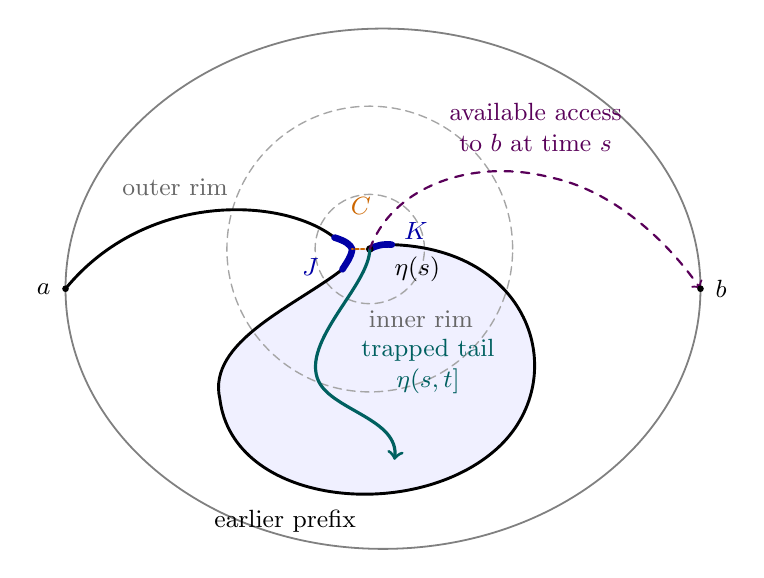
\begin{tikzpicture}[x=1.12cm,y=1.12cm,
    line cap=round,line join=round,font=\small,
    gateprefix/.style={black,line width=1.05pt},
    piece/.style={blue!65!black,line width=2.4pt},
    gate/.style={orange!80!black,line width=1.05pt,densely dotted},
    future/.style={teal!75!black,line width=1.15pt,->},
    access/.style={violet!70!black,line width=.8pt,dashed,->},
    rim/.style={black!35,line width=.5pt,dash pattern=on 3pt off 2pt}]
  \coordinate (a) at (-3.6,0);
  \coordinate (b) at (3.6,0);
  \coordinate (j) at (-.35,.45);
  \coordinate (s) at (-.15,.45);

  \path[fill=blue!6]
    (j) .. controls (-.36,.36) and (-.41,.30) .. (-.46,.22)
    .. controls (-1,-.20) and (-2,-.60) .. (-1.85,-1.25)
    .. controls (-1.70,-2.45) and (.30,-2.65) .. (1.25,-1.85)
    .. controls (2.15,-1.10) and (1.75,.45) .. (.10,.50)
    .. controls (0,.51) and (-.08,.49) .. (s)
    -- (j) -- cycle;

  \draw[black!50,line width=.65pt] (0,0) ellipse (3.6 and 2.95);
  \draw[rim] (s) circle (.62);
  \draw[rim] (s) circle (1.62);
  \node[black!60] at (.43,-.34) {inner rim};
  \node[black!60,anchor=east] at (-1.65,1.15) {outer rim};

  \draw[gateprefix]
    (a) .. controls (-2.70,1.10) and (-1.15,1.05) .. (-.55,.58)
    .. controls (-.42,.54) and (-.37,.50) .. (j)
    .. controls (-.36,.36) and (-.41,.30) .. (-.46,.22)
    .. controls (-1,-.20) and (-2,-.60) .. (-1.85,-1.25)
    .. controls (-1.70,-2.45) and (.30,-2.65) .. (1.25,-1.85)
    .. controls (2.15,-1.10) and (1.75,.45) .. (.10,.50)
    .. controls (0,.51) and (-.08,.49) .. (s);

  \draw[piece]
    (-.55,.58) .. controls (-.42,.54) and (-.37,.50) .. (j)
    .. controls (-.36,.36) and (-.41,.30) .. (-.46,.22);
  \draw[piece]
    (.10,.50) .. controls (0,.51) and (-.08,.49) .. (s);
  \node[blue!65!black,anchor=east] at (-.62,.25) {$J$};
  \node[blue!65!black,anchor=west] at (.13,.65) {$K$};

  \draw[gate] (s) -- (j);
  \node[orange!80!black,anchor=south] at (-.25,.73) {$C$};
  \fill (s) circle (1.35pt);
  \node[anchor=west] at (.02,.22) {$\eta(s)$};

  \draw[future]
    (s) .. controls (-.15,.04) and (-.94,-.60) .. (-.73,-1.05)
    .. controls (-.57,-1.38) and (.19,-1.48) .. (.13,-1.94);
  \node[teal!75!black,align=center] at (.51,-.88)
    {trapped tail\\$\eta(s,t]$};

  \draw[access]
    (s) .. controls (.11,1.17) and (1.03,1.49) .. (1.91,1.26)
    .. controls (2.57,1.12) and (3.18,.60) .. (b);
  \node[violet!70!black,align=center] at (1.73,1.83)
    {available access\\to $b$ at time $s$};

  \fill (a) circle (1.2pt);
  \fill (b) circle (1.2pt);
  \node[anchor=east] at (-3.66,0) {$a$};
  \node[anchor=west] at (3.66,0) {$b$};
  \node[anchor=north] at (-1.11,-2.40) {earlier prefix};
\end{tikzpicture}


 \caption{A small gate with both endpoints on the slit, shown
 schematically.  The endpoints of $C$ lie on an earlier piece $J$
 and a later piece $K$; $\eta(s)$ is the latest endpoint along the
 prefix.  The gate and the intervening prefix enclose the shaded
 region.  A macroscopic tail inside that region crosses the two
 rims, while at time $s$ there is an available route to the target
 on the other side of the gate.  The dashed route denotes this
 possible access, not another sampled continuation.  The annular
 radii and gate width are not drawn to scale.}
 \label{fig:tip-gate}
\end{figure}

Subdivide the curve successively into pieces of diameter less than
$b/100$, by ending a piece when it attains a chosen still smaller
fixed diameter.  Subdivide each of the two original circle arcs
into pieces with the same diameter bound.  The number of curve
pieces is stochastically bounded by
Proposition~\ref{prop:curve-tightness}.  Every gate just constructed
has its two endpoints in a pair $(J,K)$, where $K$ is a later
curve piece and $J$ is an earlier curve piece or a circle piece.
They cannot belong to the same curve piece: that would make the
loop too small to contain the excursion in
\eqref{eq:gate-excursion}.

For each ordered pair use the following revealing stopping rule
during piece $K$: stop the first time in a finite deterministic
schedule that there exists a crosscut of diameter at most $2r$
from the current tip to an earlier point of $J$.  Only non-root
slit endpoints and circle-interior endpoints are admitted.  Such
a schedule can always detect the witness above.  At fixed mesh
there are finitely many complete switch configurations.  For each
configuration exhibiting a witness choose one witness time in an
exploration-compatible clock, and take the union of those finitely
many times.  Although the selections used the full configurations,
their union is a deterministic schedule.  The detection test at
each scheduled time depends only on the current prefix.  It is
therefore a stopping rule, and it occurs no later than the witness
time for the pair in question.  If a time is inside a local piece,
only its already encountered switch is revealed.  A witnessing
crosscut at detection may also be selected deterministically from
the current history.

Let $C_1$ be this first detected crosscut for the witness pair.
We claim that its trapped region and that of $C$ agree outside
$B(\eta_n(s),b/8)$, after taking $r$ sufficiently small.  To prove
this, compare the two closed loops modulo two.  Their long common
prefix segments cancel.  The remaining prefix subarcs lie in $J$
and $K$, and the other remaining arcs are $C$ and $C_1$; in the
circle case there is also a subarc of the one circle piece $J$.
The two pieces have small diameter and are joined by a small
crosscut.  Thus this entire symmetric difference is confined to
the displayed ball.  The winding numbers modulo two of the loops
coincide outside it.  Since each loop is Jordan, its winding
parity is exactly the indicator of its trapped region there.
This proves the claim without any bound on the length or shape of
the intervening common prefix.

The far excursion in \eqref{eq:gate-excursion} consequently visits
the region cut off by $C_1$.  At detection, its tip endpoint has
access to the target side directly across $C_1$ within a ball of
radius $O(r)$.  An excursion reaching the far trapped region
either starts into that region at the detecting tip, or enters
it later through $C_1$, since the other sides of its boundary
belong to the past or the original boundary.  Both entrances
occur inside the inner ball.  The excursion therefore produces a
radial crossing, on the trapped side, from radius $4r$ to a fixed
radius, say $b/3$, about the detection tip.  Outside the inner
ball, the trapped region is bounded only by the past and the
original boundary.  Its annular components therefore cannot
connect to the target-side region without entering the inner
ball.  A route from tip to target is available on the other
side of the gate and avoids all these components, so they are
avoidable.  The argument allows repeated
future crossings of the fictitious crosscut; every such entrance
still occurs inside the inner rim.

By the disk version of Lemma~\ref{lem:macroscopic-avoidability},
the probability of this event for each ordered pair tends to zero
as $r\downarrow0$ after the mesh limit.  To finish, first use
Proposition~\ref{prop:curve-tightness} to bound the number of
pieces with arbitrarily high probability.  The resulting number
of pairs is finite and independent of $r$.  Next choose $r$ to
make the sum of their crossing bounds small, and finally choose
$y$ small enough for the crosscut construction.  This proves
\eqref{eq:tip-approximation} with the asserted order of limits.
\end{proof}

\begin{lemma}[No return from a small target cap]
\label{lem:no-return}
Let $\theta_n(r)$ be the first time $\eta_n$ enters the disk cap
$\D\cap B(1,r)$.  For every $b>0$,
\[
 \lim_{r\downarrow0}\limsup_{n\to\infty}
 \P\bigl(\operatorname{diam}
       \eta_n[\theta_n(r),\infty)>b\bigr)=0.
\]
\end{lemma}

\begin{proof}
At first entrance, the cap has not previously been visited.  It
gives a route from the tip access to the target inside a ball of
radius $O(r)$.  Stop at the entering local piece and allow a
one-step buffer.  A subsequent displacement of diameter $b$
forces a crossing from an enlarged inner rim to a fixed positive
distance, and every relevant annular component is avoidable
because of that tip-to-target route.  Apply
Lemma~\ref{lem:macroscopic-avoidability} in disk coordinates.
This is also the proof of the corresponding target-cap
Corollary in~\cite[Section ``Identification of the Dobrushin
strand'']{C}.  Initial inverse-chart continuity gives the
analogous assertion in physical coordinates.
\end{proof}
